\chapter{Data fusion for virtual visualization}

\section{Introduction}

% full field -> entire field?
The previous two chapters developed two approaches that can obtain broccoli head parts using close-range and aerial approaches. The close-range approach (Chapter 2) can obtain high-quality 3D models of the broccoli heads, while the aerial approach (Chapter 3) can obtain low-quality broccoli canopy models of the entire field. As the next step, we aim to transform and place the high-quality head 3D models into the low-quality full-field canopy models, to enable 3D virtual visualization and explanation for a more intuitive assessment of the growth status as compared to numerical statistical values. This technique is fundamental and critical for virtual farmland and digital twin technologies \citep{pylianidis_introducing_2021, slob_virtual_2023}. To the best of our knowledge, no published research has yet addressed this problem in the actual vegetable crop fields. However, several challenges need to be addressed before this goal can be achieved.

% what is backward project , what is forward projection
The first challenge is to determine a more accurate geographical location. In Chapter 3, we segmented the broccoli head on the raw images without geo-coordinates due to the low quality of the aerial model. However, converting 3D geographical coordinates (3D canopy model) to the 2D pixel coordinate (2D raw image), named backward projection, one dimension is lost and cannot be reversed. Therefore, when convecting the broccoli head segmentation results in 2D pixel coordinates back to the 3D geographical coordinate, only a ray ($Z_{cam}$) connecting the camera position ($O_{cam}$) and that point on the camera \gls{ccd} plane can be produced for each vertex (point) of broccoli head polygons (Supplementary Fig.~\ref{fig:idps1}a), rather than obtaining accurate 3D geographical points.

% convert 3D geo-coordinate to 2D pixel coordinate (backward projection); convert 2D pixel coorinate to 3D geo- is not possible, 1) information loss -> using the camera position + roatation + points on the image plane, can only get a ray, rather than a speicify 3D points. reflect to the equation in suppleate (eq.xx) need to solve xxx which is hard. The solution 1. one object from different view, and calculate the intersection points (sfm method), easy to match the polygon for each broccoli, but hard to identify the polygon vertex matches. Plus, different view may have different shapes, cannot perfectly match; 2. Find the point at which the ray intersects the surface of the model. difficulties: 对于每一条射线,都要去判断和所有的三角面是否相交,有可能遇到多个相交的三角面(如穿过叶片部分而不是花头)还需要仔细判断到底想交到了哪个面,计算量非常恐怖。一个点需要去和数十万的三角面判断关系,然后一个西兰花头就有几十个点,然后地里面有一万多的西兰花头,使得快速得到结果不太可能。
To solve the accurate 3D position, there are currently two solutions: 1) intersecting two or more rays from different perspectives to determine the 3D intersection point, which is almost the same as the \gls{sfm} process in photogrammetry; and 2) computing the intersection points between the ray and the 3D surface of the broccoli canopy model. For the first solution, matching the segmentation polygons from different perspectives for the same broccoli is not difficult, but matching each vertex is challenging. Since the shapes in different perspectives have slight differences, the vertex count may not match, let alone the vertex with "random" orders. For the second solution, it is necessary to check whether that ray intersects with all the triangular faces and calculate the intersection point if it does. On one hand, this approach requires immense computation, as a 3D broccoli canopy model typically contains millions of triangular faces, and each broccoli head polygon has dozens of vertices while there may be several thousand of them. On the other hand, a ray may intersect with multiple triangular faces, such as both the leaf and head triangular faces, so it is necessary to determine which is the actual triangular face of the broccoli head. \citet{shao_cattle_2020} optimized this approach by projecting the 3D triangular faces onto the raw image to generate a depth image in order to resolve the dimension loss, which is still computationally intensive for rendering each pixel, and code is not available.

% 所以在第三章中,使用的规则是,根据grid定点在两个坐标中的位置,直接使用projective transformation, 进行变换,这样计算比较迅速,而且基于西兰花田地的特点(一个起伏变化不是很大的平地),能大体上保证变换后尺寸比例的正确性,并不影响head traits的计算;但是由于视角等细微的变化,导致位置上的正确性不是很好(Fig.1.1); 为了能更准确的实现可视化,把西兰花头更精准的放回到地里面,需要对这个位置变幻进行进一步的优化
In Chapter 3, we proposed a simplified solution. Since only the actual size is required, rather than accurate positions for that chapter, we assumed that the relative sizes of the broccoli polygon and the grid boundary remain unchanged in the two perspectives (Fig.~\ref{fig:xrs1}a-b). In practice, we applied projective transformation, which directly stretches the image according to the \gls{roi} vertices (blue broken lines in Fig.~\ref{fig:xrs1}). Therefore, although the positions may not fit perfectly due to slight angle variations in perspectives between the raw image (Fig.~\ref{fig:xrs1}a, with a slight slant) and the \gls{dom} (Fig.~\ref{fig:xrs1}b, the vertical view), we can obtain the actual geographical sizes of broccoli heads, which is enough for the objective of Chapter 3. However, the position accuracy of this method may not be enough for the 3D visualization objective of this chapter and requires further optimization.

\begin{figure}[htb!]
  \begin{center}
    \resizebox{\textwidth}{!}{
      \includegraphics{figures/xrs/challenges.pdf}
    }
  \end{center}
  \caption[Challenge to forward results from pixel coordinate to geographical coordinate]{
    Challenge to forward results from (a) pixel coordinate on raw image to (b) geographical coordinate on \gls{dom}. The red polygons are broccoli head segmentation results while the blue broken lines are the boundary of the current plot grid. (b) shows the projective transformation on the grid vertices has slight deviations.
  }
  \label{fig:xrs1}
\end{figure}

% 另外,由于地里面的尺寸和我们破坏性采样的西兰花,尺寸并不能完美的匹配,因此还需要针对尺寸进行适当的变幻,比较常用的方法是建立一个样地尺寸-db尺寸的线性回归模型,但是由于细小的差距,在我们预实验中,效果并不理想。而选择不同回归模型需要大量的时间去尝试来找到表现最好的,因此采用Auto-ml来节省时间。
The second challenge is how to properly match and adjust the close-range broccoli models to the aerial results. The first step is calibration, which makes the morphological traits of broccoli heads measured from the aerial closer to the ``ground truth''. For the model calibration of complex cases, compared to linear regression, the machine learning models such as \gls{svm} and \gls{rf} were often used by several studies \citep{nguyen_uav_2023, lu_assessment_2022}. However, the selection and tuning of the machine learning model also pose a challenge. \citet{wang_landscape_2019} reported that \gls{cart} outperformed \gls{svm}, \gls{rf}, and \gls{gbdt} on plant classification tasks. However, \citet{han_drone_2021} found that \gls{svm} performed best on flower classification tasks compared to \gls{rf}, \gls{cart}, \gls{lda}, and \gls{knn}. Furthermore, \citet{han_modeling_2019} reported that \gls{rf} yielded better results on biomass prediction than \gls{mlr}, \gls{svm}, and \gls{ann}. These studies indicate that the performance of different machine learning algorithms varies depending on the task at hand. From our experience, model selection is an empirical process that may require extra time to compare mainstream algorithms. To be effective in practice, the demand for an optimized machine learning system that can automatically choose the algorithm and set its hyperparameters for non-experts is increasing \citep{feurer_efficient_2015}. The next step after calibration is converting the broccoli heads in the database and fitting them to the calibrated morphological traits. Since we only destructively sampled around 200 broccoli heads to obtain high-quality models, we still cannot cover all shapes of broccoli heads grown in the entire field. Therefore, template matching and transformation methods should also be developed.

In this chapter, we aimed to develop a 3D virtual visualization technique that can fuse high-quality 3D head models, obtained using close-range reconstruction (Chapter 2), with full-field canopy models, obtained through aerial photogrammetry (Chapter 3). Our objectives were to: 1) develop an optimized method to obtain more accurate geographical locations of segmented broccoli heads from raw images; 2) use the latest \gls{automl} technique to generate a calibration model for aerial measurements of head traits; 3) develop a template matching method that can quickly find the broccoli model in the database with the smallest difference to the calibrated traits; 4) apply geometric transformations to the matched head 3D model template to reduce differences to  the calibrated traits; and 5) develop a visualization script to display the results in 3D.

\section{Methods and Materials}

The general workflow for 3D visualization can be summarized into three main parts: 1) obtain the accurate geographical position of each broccoli head from the aerial approach (optimize Chapter 3); 2) calibrate the morphological traits of the broccoli head from aerial measurements, then locate and transform the nearest template from the high-quality broccoli head database (produced by Chapter 2); and 3) fuse the close-range and aerial results and visualize them in 3D.

\subsection{Data collection and preprocessing}

The broccoli data used in this chapter was obtained in the spring of 2022 (Chapter 2) and the detailed plot conditions were introduced in Subsection \ref{sec:2022plot}. The high-quality 3D model of 189 destructively sampled broccoli heads was obtained from the workflow in Subsection \ref{sec:3ddb}. Additionally, the field 3D model of the aerial photogrammetry from this year was obtained from the workflow introduced in Subsection \ref{sec:cp3data}. However, we changed the aerial photogrammetry software from Pix4DMapper Pro (Pix4D, S.A., Prilly, Switzerland) to Agisoft Metashape (Agisoft LLC, St. Petersburg, Russia). Then, the same workflows for broccoli detection (Subsection \ref{sec:detect}) and segmentation (Subsection \ref{sec:seg}) were applied to obtain the broccoli head polygons from the raw images. The morphological traits of broccoli heads from the close-range database and the aerial survey were calculated by Subsection \ref{sec:mte} and Subsection \ref{sec:pheno}, respectively.

\subsection{Optimized positioning}

Inspired by the depth image rendering proposed by \citet{shao_cattle_2020} and the projective transformation used in Chapter 3, a control point array covering the \gls{roi} and the broccoli segmentation results (Fig.~\ref{fig:xrs2}a) was generated in geographical coordinates on the \gls{dom}. These control points were then backward projected onto the raw images (Fig.~\ref{fig:xrs2}b) and the piecewise affine transformation was used to revert coordinates according to these control points in both coordinates. \citet{pitiot_piecewise_2006} previously applied this technique to register biological images for volume reconstruction. This transformation was applied to the broccoli head segmentation results to obtain more accurate geographical positions.

\begin{figure}[htb!]
  \begin{center}
    \resizebox{\textwidth}{!}{
      \includegraphics{figures/xrs/transform_cp_220331_114_DJI_0289.pdf}
    }
  \end{center}
  \caption[Control points between geographical coordinates on DOM and the pixel coordinate on raw image]{
    Control points between geographical coordinates on DOM and the pixel coordinate on raw image. The blue broken lines are the \gls{roi} boundary of the current grid, the red dots are the control points.
  }
  \label{fig:xrs2}
\end{figure}

After converting the broccoli head segmentation results to the graphical coordinates, the center of the head was calculated in order to position the high-quality 3D head models from close-range database. The circle fitting procedure described in \citet{blok_image_2021} was applied to the convex hull of the broccoli head to determine its center, which partially solves the issue of leaf occlusion to some degree. To obtain the height (z) values of that center point, the mean value of all points in the head region $\geq$95th percentile height was calculated. 

\subsection{Template matching and transformation}

% calibration by auto ML
Before performing template matching and transformation, a calibration model is required to improve the performance of the system. This model should be trained by relating the aerial morphological traits to the close-range morphological traits. Since we sampled the close-range broccoli heads destructively after the aerial survey, we were able to obtain such data pairs. These data pairs were divided into training data and validation data with a 4:1 ratio. The training data was used to train an \gls{automl} multi-output regression model \citep{feurer_auto-sklearn_2020} to calibrate the morphological traits from aerial surveys, while the validation data was used to assess the calibration model's performance.

The next step is to find the template broccoli head from the close-range database. We modified the normalized cross-correlation of image template matching \citep{yoo_fast_2009}, which helped us find the closest 3D head template with the smallest differences:

\begin{equation}
  \bar{j} = \mathop{argmin}_j 
    \sum_i^{n} \sqrt{\sum_{i,j}^{m} \left| T_i - D_{i,j} \right| ^ 2}  
\label{eq:xrs1}
\end{equation}

\noindent
where, $T_i$ is the i-th of calibrated morphological traits of the current aerial broccoli head with a total number of n (in our data, $n=6$, including length of major axis, length of minor axis, width of minimum area rectangle, length of minimum area rectangle, area, and convex area); $j$ is the j-th of broccoli head in the close-range template database with a total number of $m$ (in our data, $m=189$); $D_{i,j}$ is the i-th of morphological traits of j-th of broccoli head in the template database; $\bar{j}$ is the j-th of broccoli head that finally matched.

% geometric transforming
After obtaining the closest template, the ratios between the calibrated values and template values were used as the zoom ratios for template transformation. To be more specific, the width and length of the minimum area rectangle were used as the horizontal and vertical zoom ratios along the minor and major axes, respectively.

\subsection{3D virtual visualization}

% the open3d is used to visualize.. how to segment to small parts, and how to load mesh and display.
Since the triangular face count of each close-range high-quality broccoli head model is often over 50,000, it is not feasible to directly render the entire field with thousands of broccoli. Instead, we render one \gls{roi} grid at a time to decrease the demand for computational resources. The EasyIDP package (\url{https://github.com/UTokyo-FieldPhenomics-Lab/EasyIDP}, Supplementary material \ref{spp:backward}) was used to crop the \gls{roi} broccoli canopy 3D point cloud (by aerial photogrammetry), and the transformed broccoli heads were placed at the 3D geographic head center points. The Open3D Python package \citep[\url{https://github.com/isl-org/Open3D}]{zhou_open3d_2018} was used to process and visualize the 3D models. The code and script for data processing and interactive visualization can be found at \url{https://github.com/UTokyo-FieldPhenomics-Lab/BroccoliHead3D.ipynb}.

\section{Results}

The aforementioned workflow demonstrated the feasibility of most \gls{roi} grids, particularly those with dates close to the optimal harvest date with larger broccoli head sizes. In this section, some representative examples were used to illustrate.

\subsection{Optimized positioning}

Figure~\ref{fig:xrs3}a shows the segmentation results of broccoli on the raw image, while Figure~\ref{fig:xrs3}b displays a comparison between the optimized positioning method (blue polygons) and the one used in Chapter 3 (red polygons). The broccoli heads in the bottom row (Fig.~\ref{fig:xrs3}a) correspond to the left column in Figure~\ref{fig:xrs3}b, which has an almost vertical perspective and thus conforms to the position in geographic coordinates. On the other hand, in the top row of Figure~\ref{fig:xrs3}a (corresponding to the right column in Fig.~\ref{fig:xrs3}b), the perspective is not perfectly vertical. As mentioned in the introduction of this chapter, the method used in Chapter 3 (red polygons) shows clear deviation, while the proposed optimized method (blue polygons) still accurately displays on the geographical positions of the broccoli heads.

\begin{figure}[htb!]
  \begin{center}
    \resizebox{\textwidth}{!}{
      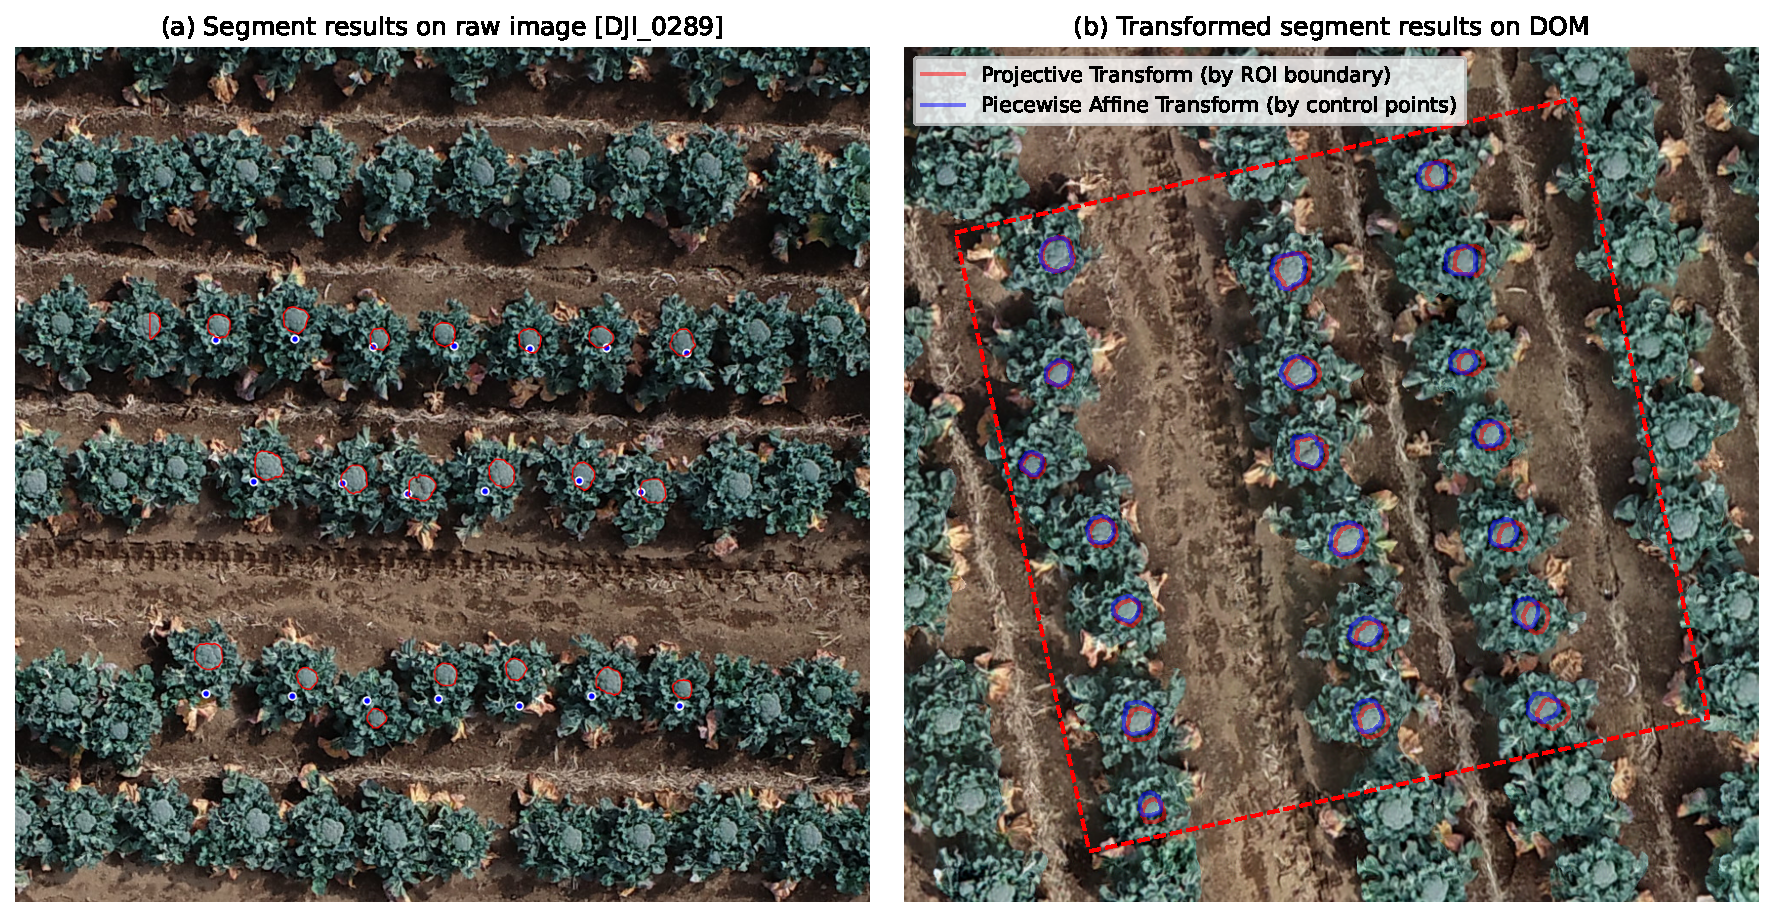
\includegraphics{figures/xrs/trans_compare_220331_114_DJI_0289.pdf}
    }
  \end{center}
  \caption[Head segmentation forward location comparison between projective and piecewise affine transformation]{
    Head segmentation forward location comparison between projective (in Chapter 3) and piecewise affine transformation (this chapter). (a) is the head segmentation results on the raw image. They are forward transformed to corresponding positions on the \gls{dom} using two different transformations.
  }
  \label{fig:xrs3}
\end{figure}

\subsection{Template matching and transformation}

The full pairwise data was split into training and testing sets using a 4:1 ratio, and the calibration \gls{automl} model was trained on the training set only. The components of the calibration \gls{automl} model are shown in  Table~\ref{tbl:xrs1}. Three \gls{rf} models (IDs 72, 73, and 69) with larger ensemble weights ($\geq 0.20$) were selected, as well as two \gls{knn} models (IDs 67 and 20). These models were combined as a mixture model, and the results output by each model were weighted according to their respective weights to obtain the final result.

\begin{table}[htb]
  \caption{The components of AutoML calibration model}
  \label{tbl:xrs1}
  % \begin{adjustwidth}{-0.05\textwidth}{-0.05\textwidth}
    \begin{center}
      \begin{tabular}{cccc}
        \hline
        \textbf{model id} & \textbf{rank} & \textbf{ensemble weight} & \textbf{type}       \\ \hline
        72                & 1             & 0.22                     & random forest       \\
        55                & 2             & 0.08                     & random forest       \\
        2                 & 3             & 0.02                     & random forest       \\
        73                & 4             & 0.28                     & random forest       \\
        69                & 5             & 0.24                     & random forest       \\
        67                & 6             & 0.06                     & k nearest neighbors \\
        20                & 7             & 0.10                     & k nearest neighbors \\ \hline
        \end{tabular}
    \end{center}
  % \end{adjustwidth}
\end{table}

The validation was conducted on the remaining testing dataset. According to the results (Fig.~\ref{fig:xrs4}), the calibration model obtained good correlation ($R^2 \geq 0.84$) between calibrated values and validation values for the six morphological traits. Compared to the morphological traits without calibration (red), the calibrated traits (blue) have a higher correlation and lower \gls{rmse}. The calibrated traits (solid regression line) are closer to the standard line, which means that the \gls{automl} calibration model corrects the underestimated trend (mainly due to occlusion for small broccoli heads) of aerial measurements.

\begin{figure}[htb!]
  \begin{center}
    \resizebox{\textwidth}{!}{
      \includegraphics{figures/xrs/validation4automl.pdf}
    }
  \end{center}
  \caption[Validation for the AutoML calibration model]{
    Validation for the AutoML calibration model.
  }
  \label{fig:xrs4}
\end{figure}

The calibration also contributed to better template-matching results. Take one plot with variable broccoli head sizes (ranging from 10cm to 22cm) as an example (Fig.~\ref{fig:xrs5}). The calibrated results showed higher correlation and lower \gls{rmse} compared to those without calibration. The distribution was also closer to the standard line, which could result in a smaller transformation for the templates.

\begin{figure}[htb!]
  \begin{center}
    \resizebox{\textwidth}{!}{
      \includegraphics{figures/xrs/aerial_matched_compare_220405_29.pdf}
    }
  \end{center}
  \caption[The closest matched broccoli head template 3D model]{
    The closest matched broccoli head template 3D model to each aerial segmentation results. Different colors represent different broccoli heads.
  }
  \label{fig:xrs5}
\end{figure}

\subsection{3D virtual visualization}

Figure~\ref{fig:xrs6} shows a representative plot grid for 3D virtual visualization with varying broccoli head sizes before the optimal harvest date. Figure~\ref{fig:xrs6}a shows the broccoli head segmentation results on the raw image, while Figure~\ref{fig:xrs6}b shows the aerial broccoli canopy 3D point cloud models. It was almost impossible to observe the broccoli head directly on the point cloud model (Fig.~\ref{fig:xrs6}b). By using the workflow proposed in this chapter, the high-quality 3D models were transformed and accurately placed into the point cloud model with low resolution (Fig.~\ref{fig:xrs6}c). Figure~\ref{fig:xrs6}d shows another perspective of the 3D visualization, and Figure~\ref{fig:xrs6}e shows the model details after zooming closer. Some of the broccoli heads touched the plot boundary (two on the top right and one on the bottom left, Fig.~\ref{fig:xrs6}c) and did not show up; because we defined the lower and right boundaries as belonging to the neighbor grids. These broccolis showed up in that grid.

\begin{figure}[htb!]
  \begin{center}
    \resizebox{\textwidth}{!}{
      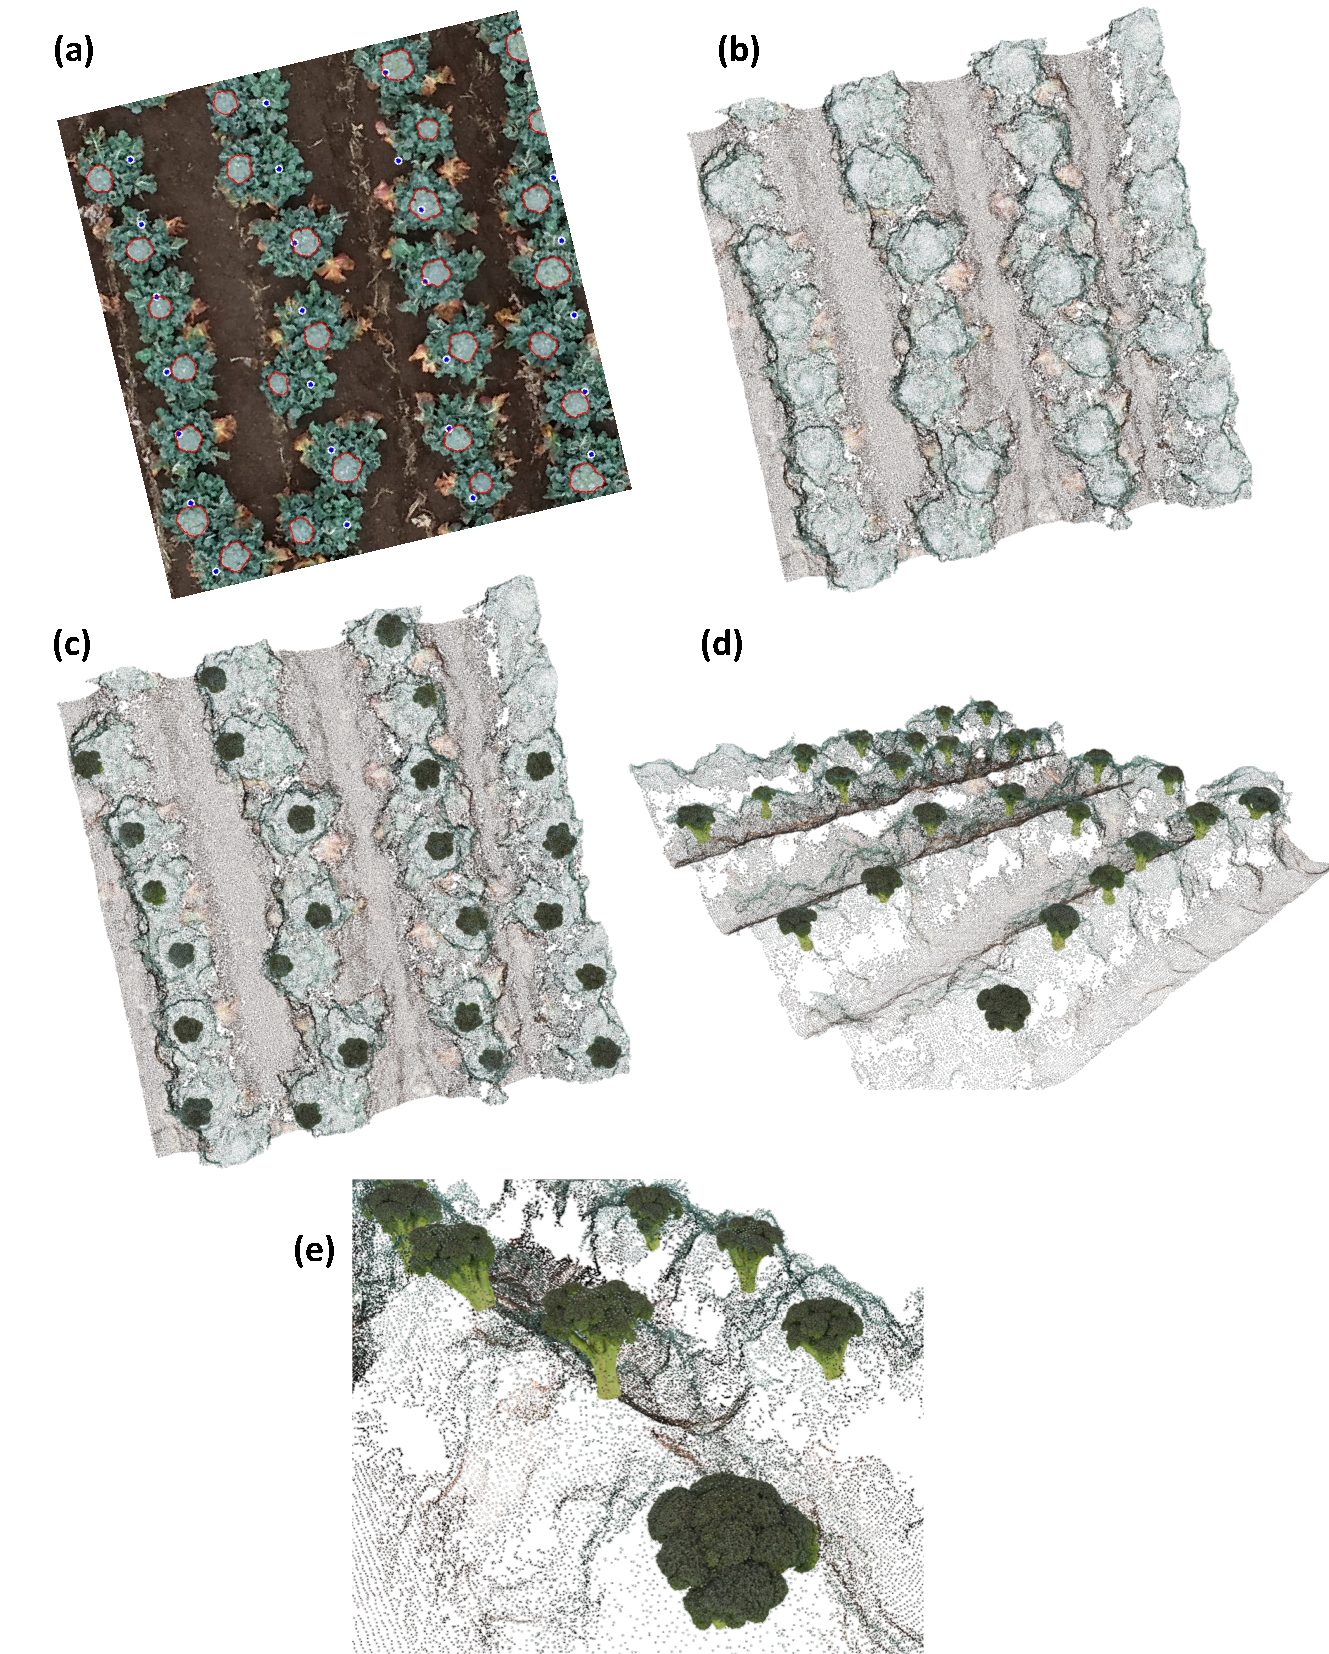
\includegraphics{figures/xrs/open3d_view.pdf}
    }
  \end{center}
  \caption[One example of 3D virtual visualization for optimal harvest date]{
    One example of 3D virtual visualization for optimal harvest date; (a) is the broccoli head segmentation results on raw aerial image; (b) is the top view of original aerial 3D point cloud models for broccoli canopy; (c) is the top view of canopy model with matched high-quality 3D broccoli heads; (d) is the side view; and (e) is the zoom in detailed view.
  }
  \label{fig:xrs6}
\end{figure}

\section{Discussion}

The 3D virtual visualization of broccoli heads introduced in this chapter provides, for the first time, a data fusion method that combines the advantages of high-quality close-range reconstruction (Chapter 2) and high throughput aerial survey (Chapter 3). We observed that the proposed method, including optimized positioning (Fig.~\ref{fig:xrs3}), automated machine learning calibration (Fig.~\ref{fig:xrs4}), and template matching and transformation (Fig.~\ref{fig:xrs5}), had clear improvements compared to previous or controlled methods in both correlation and \gls{rmse}. The final 3D virtual visualization (Fig.~\ref{fig:xrs6}) shows the feasibility of this technique as a fundamental and critical component for virtual farmland and digital twin for future studies.

% 即使不进行校准(因为涉及到实际破坏性采样),
Obtaining paired training data (the same broccoli plant appears in both close-range and aerial view) for model calibration is a time-consuming and challenging process. It involves careful verification of the field and destructive sampling ids to ensure matching accuracy, as well as data cleaning to remove outliers. For example, in this experiment, due to the complexity of field conditions, the segmentation results for 3 broccoli heads on the original image were not perfect, resulting in great differences in morphological traits between aerial and close-range views. Adding them to our pre-experiment would decrease the model's correlation to only around 0.5. After removing these outliers, the calibration model correlation ($R^2$) increased to over 0.84 (Fig.~\ref{fig:xrs4}). However, this does not mean that the process is mandatory when applied to new broccoli fields. Due to the similarities in the growth and occlusion of broccoli, the model we trained can theoretically be transferred to new broccoli fields for calibration. In addition, based on our comparison results (Fig.~\ref{fig:xrs4}), even without calibration, the \gls{rmse} is $\leq$ 0.97 $cm$ for length and $\leq$ 13.6 $cm^2$ for the area.  We can still find corresponding templates in the template database for transformation with an acceptable level of error (RMSE $\leq$ 3.1 $mm$ for length and $\leq$ 2.76 $cm^2$ for head area) without calibration. But we need to consider that smaller broccoli may be underestimated. Since the optimal harvesting date usually consists of larger broccoli, the impact of this underestimation is still acceptable. It was suggested for further experiments to evaluate the transferability of the \gls{automl} calibration model and the impact of skipping the calibration in new broccoli fields.

As a pioneer study in its early stage, we have to admit that the proposed method in this chapter has some limitations. 
Firstly, the current visualization is still rough and limited by performance, which requires breaking down the entire field into smaller parts for 3D virtual visualization. It was suggested to use game engines to develop a user-friendly \gls{gui}, or even a \gls{vr} or \gls{ar} interface. Also, integrating all the methods in the thesis into a software product for users to conveniently apply in their field should be considered. 
Secondly, the occlusion problem has not been completely solved yet. The current method of addressing occlusion is through \gls{automl} model calibration, but the statistic-based calibration is difficult to surpass the shape-based occlusion repair. \citet{blok_image_2021} proposed an approach based on \gls{orcnn} to repair missing parts. It requires a camera with its position fixed over a broccoli head. Then a fully exposed broccoli head image was collected as the ground truth and leaves were used to create training data with varying degrees of occlusion. Further adjustments are needed for the application of drone imagery in the future. 
Thirdly, there is only one cultivar in the close-range 3D broccoli head model database, which is not sufficient to reflect the differences between different broccoli cultivars. Further cooperation with farms is needed to acquire more high-quality 3D models of different broccoli cultivars for further expansion of the database. 
Fourthly, the current broccoli placement strategy simply performs geometric transformations and places the broccoli directly back to the center point, which cannot guarantee a perfect fit of the broccoli crowns to that of 3D point cloud of broccoli canopy from the aerial photogrammetry. Additionally, the base of the model is suspended in the air rather than connected to the soil. For some inclined growing broccoli, it is noticeable that the stem does not bend towards the soil mound, which does not truly reflect the actual growth situation. In the future, matching and more delicate transformation should be considered with the broccoli crown surface of the aerial model, as well as the relative growth relationship between the stem and the soil, to achieve a more realistic display effect.
Fifthly, simply expanding the database of destructive sampling is not sufficient to achieve the above goals, as it involves many complex structural transformations and combinations, thus a  virtual broccoli model controlled by several parameters needs to be developed. Similar to the virtual maize model implemented in \citet{cieslak_l-system_2021}, which can use parameters to change the details of plant structure. It was suggested to develop such a procedural model for broccoli heads. 

\section{Conclusions}

The work in this chapter aimed to develop a 3D virtual visualization technique that can fuse high-quality head 3D models (from Chapter 2) into low-quality full-field canopy models (from Chapter 3). By using piecewise affine transformation, \gls{automl} calibration model, and template matching and transformation, a 3D virtual visualization system was developed to visualize the broccoli head sizes at their field positions. The statistical analysis supports the improvements of the proposed method in geographical locations and broccoli morphological traits. The proposed 3D visualization system offers a great opportunity for virtual farmland and digital twin technology, which can provide a more intuitive feeling of growth status compared to numeric statistical values.